%========================= Algorithm Design =========================
\label{Algorithm Design}
This chapter presents how the application is designed at a logical level and describes the 
main algorithms and techniques which are combined and used by the implementation.

\section{Planarity testing}

The first algorithm used by the application is the planarity testing method known as "vertex addition". In 
order to properly present this algorithm, we must first introduce the necessary notions regarding graph planarity 
and methods of testing this property.

\subsection{Planarity property and criteria}

A given graph \emph{G=(V,E)} is planar if it can be drawn on a plane and its edges never cross each other, i.e. they 
intersect only at their endpoints. This type of drawing is also known as a planar embedding of the graph.

In order to determine if a graph possesses the planarity property, a series of theorems and criteria have been 
stated over the years. Amongst the first of these criteria is a theorem published by the Polish mathematician 
Kazimierz Kuratowski\cite{kuratowski} in 1930. The theorem deals with subdivisions, i.e. graphs which result from inserting vertices 
into edges. It states that a planar graph shall not contain a subdivision of the forbidden graphs K5(the complete 
graph on five vertices) or K3,3(complete bipartite graph on six vertices, three of which connect to each of the other 
three, also known as the utility graph). It is formulated as follows:\\

\textit{
A finite graph is planar if and only if it does not contain a subgraph that is a subdivision of K5 or K3,3 .
}

Another important theorem which deals with planarity was formulated by the German mathematician Klaus Wagner. 
This theorem takes into consideration graph minors instead of subdivisions. A graph H is called a minor of a given 
graph G if H is obtained by deleting vertices and edges or by contracting edges. The Wagner theorem states that 
a finite graph is planar if and only if it does not have K5 or K3,3 as a minor.

While these theorems manage to correctly define the planarity problem in a mathematical way, they are not optimal 
criteria to use in practice. The main reason is efficiency: we would like the complexity of such an algorithm 
to be linear - O($n$). In practice, there are other theorems and criteria which fit in the linear complexity. For 
example, given a finite, connected planar graph with v the number of vertices, e the number of edges and 
f the number of faces (regions bounded by edges, including the outer, infinitely large region), the following 
hold true:
\\ 
\\ \textit{Theorem 1: If $v \geq 3$ then $e \leq 3v-6$;}
\\ \textit{Theorem 2: If $v \geq 3$ and there are no cycles of length 3, then $e \leq 2v-4$;}
\\ \textit{Theorem 3: $v - e + f = 2$} (Euler's formula).
\\ 
\\ Unfortunately, these theorems are only necessary conditions, not sufficient conditions. They can only be used to 
prove that a graph is not planar; they cannot prove that a graph is planar.

\subsection{Vertex addition method}

The edge addition algorithm is the result an intensive research started in the 1960s by Abraham Lempel, Shimon Even
and Cederbaum. They created an algorithm to determine whether a graph is planar or not and embed it in the plane in 
O($n^{2}$) time. Later on, Even and Tarjan developed a method to generate the st-numbering of a graph in linear O(${n}$) time.

\begin{figure}[ht] \centering
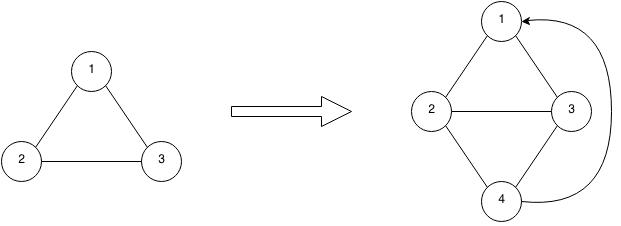
\includegraphics[width=0.75\textwidth]{img/algdesing/st_numbering.png}
\caption{St-numbering representation of the G(3,3) graph} \end{figure}

An st-numbering\cite{even1976computing} of a graph G is a subgraph H which has a set of properties, as follows. First, nodes in G are numbered. 
Then the vertex with the lowest number is designated as source vertex, \emph{s}, and the one with the highest number 
is designated target, \emph{t}. All the remaining vertexes which are not the source or target must be connected to a 
vertex numbered lower than them, and a vertex numbered higher than them. In order to achieve this configuration, the 
subgraph H may add additional nodes to the graph G.

Finally, Kellogg Booth and George Lueker created a data structure which represents the possible embeddings of a graph 
(or, in practice, induced subgraphs of a graph) called a \emph{PQ-tree}. Using this data structure and the previous methods, 
they managed to created a linear time algorithm to determine planarity and possible embeddings. We will next present 
the general steps of an implementation of the Vertex addition method as proposed by Norishige Chiba and Takao Nishizeki\cite{chiba}.

First, it computes the st-numbering of the given graph. It then creates a PQ-tree which contains only one P node, the 
source, and all the other nodes are leaves. Next, a loop is entered which, for every leaf node, shall perform two steps:

\begin{itemize}
\item A reduction step which attempts to gather all matching leaves into a P node which respects the st-numbering. If this 
step fails, then the graph is not planar.
\item A vertex addition step, in which full nodes are replaced by a single P node and all the neighbours of that node 
numbered higher than itself are added as leaves.
\end{itemize}

\begin{lstlisting}[caption={Vertex addition algorithm as proposed by Chiba and Nishizieki}]
PROCEDURE PLANAR(G);
BEGIN
st_numbering(G);
make_PQ_tree(s); //construct PQ-tree with root in s
FOR v := 2 to n:
	BEGIN
		// start of reduction step
		reduction = gather_leaves(template, subtree_root);
		IF reduction == FAILED:
		THEN BEGIN
			set_planar(G) = FALSE;
			RETURN
		END
		// end of reduction step
			
		// start of vertex addition step
		replace_full_node(PQ-tree, P-node)
		FOR t in neighbours(v):
			BEGIN
				IF st_number(t) > st_number(v):
				THEN BEGIN
					add_to_PQ_tree(t);
				END
			END
		// end vertex addition step
	END
set_planar(G) = TRUE;
END
\end{lstlisting}



Figures 3.2 to 3.4 below present the steps of this algorithm applied on a graph G(3,3).

\begin{figure}[ht] \centering
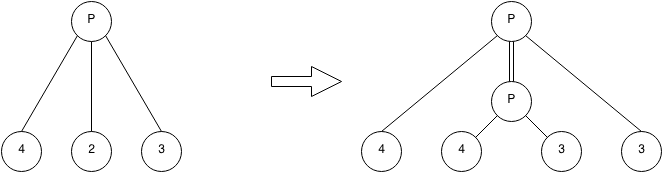
\includegraphics[width=0.75\textwidth]{img/algdesing/vertex_reduction_step_1.png}
\caption{The initial representation of the graph and the configuration after one merge step} \end{figure}

\begin{figure}[ht] \centering
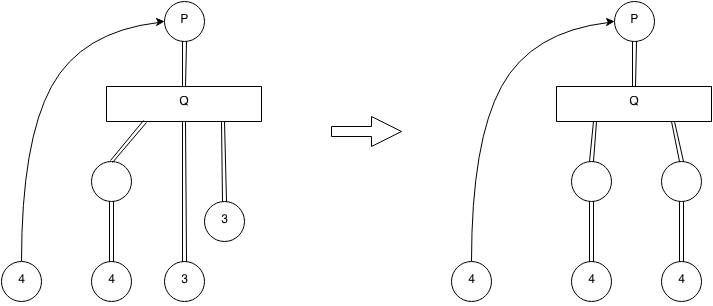
\includegraphics[width=0.75\textwidth]{img/algdesing/vertex_reduction_step_2.png}
\caption{Graph representation after two more reduction steps.} \end{figure}

\begin{figure}[ht] \centering
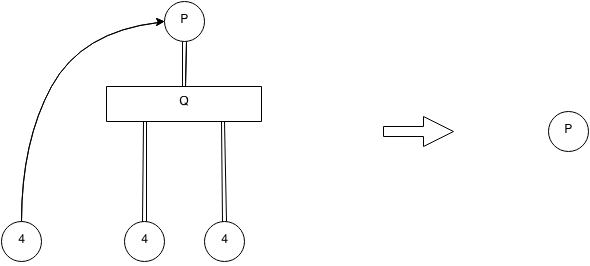
\includegraphics[width=0.65\textwidth]{img/algdesing/vertex_reduction_3.png}
\caption{Complete PQ-tree representation and the final merge into a single P node} \end{figure}

\section{Graph placement}

Graph placement refers to assigning a position (set of coordinates) to each node of the graph in the space where 
the graph has to be represented.

We saw in the previous chapter that algorithms which determine if a graph is planar can also generate its 
embeddings. However, this is not the same as actually drawing the graph. In reality, we are constrained by the 
limitations of the space in which we want to draw the diagram. Therefore, even though we know that a possible 
arrangement of the nodes will allow us to represent the graph in a plane, we cannot be certain that the 
representation is feasible or understandable. Furthermore, one may want to draw even graphs which are not planar, 
knowing that two or more of its edges will cross one another.

For this reason, a logical positioning of each node in the given plane is required. This step greatly facilitates 
the routing process and also helps reduce the time and complexity of said operation.

Commonly used methods which are also incorporated in the solution proposed by this thesis include grid placement and 
force directed graph-drawing. We shall continue by presenting these methods in the following sections.

\subsection{Grid placement}

Grid placement\cite{de1990draw} is one of the most popular and most used techniques by diagram-drawing algorithms. It splits the space in 
which the representation is done into a grid and then starts placing the nodes in a certain order. Different approaches 
can be found here, depending on the type of the graph. 

Trees are often placed in layers. The root of the tree is first fixed on an edge of the grid, and then each level of the tree 
visited in breadth-first order forms a layer of nodes. Layers can be arranged vertically or horizontally, depending on the implementation.

\begin{figure}[ht] \centering
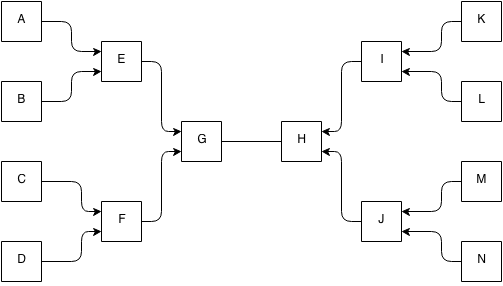
\includegraphics[width=0.65\textwidth]{img/algdesing/grid_example.png}
\caption{Example of a tournament structure organized as a grid.} \end{figure}

More general graphs may also follow this pattern, by computing the spanning tree\cite{graham1985history} of the graph and placing nodes as stated above, 
starting with the spanning tree's root. Other approaches for general graphs may place and pin the node with the highest number of 
connections in the middle of the grid.

The advantages of this method are represented by its ease of implementation, small consumption of resources and low complexity. A main drawback 
is that it generally interferes with the routing process and does not facilitate it. It also poses the risk of drawing planar graphs as though 
they were non-planar, i.e. intersecting various edges.

\subsection{Force directed graph-drawing}

Force directed drawing\cite{fruchterman1991graph} is a technique which borrows concepts from physiques. In order to apply this method, one must model the graph as a 
physical system in which elements (nodes) interract with each other through forces. Connected nodes will be pulled towards each other by 
attraction forces (such as spring forces base on Hooke's Law), while unrelated nodes reject each other (similar to electrically charged particles
according to Coulomb's Law). These forces are applied continuously until the system reaches stability.

Using such a technique will yield a graph placement which has the strongly connected nodes pulled in the middle of the assigned drawing spaced, while the 
individual or loosely connected nodes are pushed towards the edges. The same holds if the graph is split into multiple independet connected components: 
the nodes of each component shall be pulled towards each other, while the individual components will reject one another.

\begin{figure}[ht] \centering
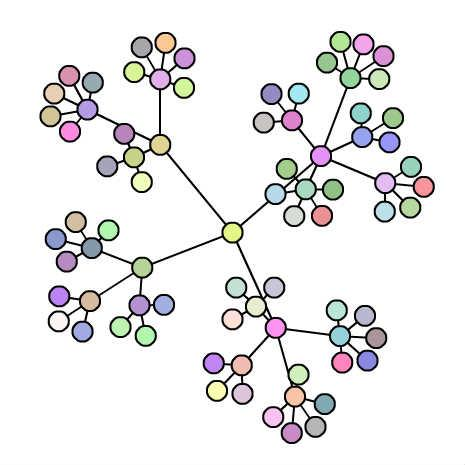
\includegraphics[width=0.5\textwidth]{img/algdesing/force_directed_example.jpg}
\caption{A force-directed graph layout with a central node and multiple connected components.\protect\footnotemark} \end{figure}
\footnotetext{Image taken from \url{http://wonderfl.net/}}

This approach is better suited to ease the routing process and reduce its time and complexity. It is less likely that planar graphs shall be 
improperly drawn and routes will be shorter and clearer. However, unlike Grid placement, it is an iterative process which may take considerable 
amounts of time to reach stability, while also consuming more resources.

\section{Edge routing}

The final step in drawing a diagram or a graph is represented by edge routing. Its purpose is to highlight the connections and dependencies between 
nodes via a set of lines which add up to make paths between nodes. An important aspect is that paths must not cross over other nodes, even though 
this may increase the length of a path by adding extra segments to it. Depending on how the paths are represented, edge routing may be:

\begin{itemize}

\item Shortest path routing: Nodes are connected only by straight which go directly from the source to the destination. In some implementations, it 
is acceptable for these lines to cross other nodes, while in others extra segments are added in order to go around obstacles.
\item Arc routing: This approach represents paths as arcs. Nodes are usually placed in a linear layout (all nodes are placed on the same axis) and 
each edge is considered a diameter line for a circle. Then an arc of corresponding length is drawn to join the pair of nodes.
\item Orthogonal routing: In orthogonal routing, paths are composed only of vertical and horizontal lines, joined by 90 degree bends. While it is 
not the most efficient method with regards to the space occupied by the drawing, it does provide clear and direct paths which do not cross over other elements.

\end{itemize}

\subsection{Rule-based genetic routing algorithm}

Having presented the range of algorithms which help achieve the goal of representing and drawing diagrams, we can now explain and exemplify how 
the implementation of this thesis works. We shall go through each of the three steps: planarity testing, node placement and edge routing, explaining in detail the design of each level.

The proposed implementation starts by testing the planarity of the input graph using the criteria derived from Euler's theorem. These theorems are 
applied first because of their reduced complexity and because all the needed information is computed when the graph is first constructed. Should the 
result be negative, there is sufficient information to decide that the graph is not planar and that the drawing will have crossing edges. 
If, otherwise, the result is positive, we know that the theorems are only a necessary condition, not a sufficient one. At this point, the PQ-tree 
algorithm is applied to thoroughly decide if the graph is planar.

With the planarity property of the graph decided, the algorithm proceeds to the placing step. Here, the nodes will be assigned positions in the 
drawing space (the canvas) based on certain criteria. This can be achieved in two ways: if the graph is a planar graph with the number of nodes 
below a specified threshold, the layout shall be a grid. Otherwise, the main routing algorithm is applied. This selection of layout models ensures 
that the application does not complicate a problem which presents an easy solution.

\begin{figure}[ht] \centering
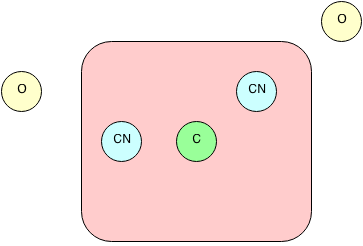
\includegraphics[width=0.5\textwidth]{img/algdesing/centralnode.png}
\caption{The reserved area around the central (C) node. Its neighbours (NC) are permitted inside, but other nodes (O) are not.} \end{figure}

In the case of the rule-based algorithm, during the first step, as seen in grid placing, the node with the highest number of connections is 
placed in the center of the canvas. Then, a certain amount of canvas space is reserved around this node. The central node's neighbours 
shall be placed in this area in a random order, and no other node may be placed in this area. This step ensures that the random factor is mostly eliminated 
 for this group of nodes and a certain consistency is kept amongst consecutive drawings of the same graph. All the other nodes are placed randomly in the remaining area.

At this point, notions from genetic algorithms are introduced. The graph is considered a population and each node represents an individual. For the 
remaining steps, each individual shall be evaluated by a fitness function and suffer modifications depending of the result. In order to change and evolve 
the population, the position of a node shall be modified in the recombination step. Each node outside the reserved area shall generate, along with its neighbour closest to 
the center, a new pair of nodes which are either closer to each other (attracted) or further apart from each other (rejected), as described by the force-directed method. This step shall 
continue until a certain number of steps has been exhausted (we have explored the maximum allowed samples of populations) or the system has reached stability.

\begin{figure}[ht] \centering
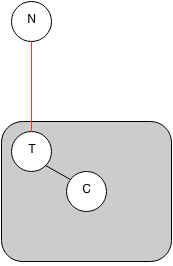
\includegraphics[width=0.2\textwidth]{img/algdesing/recombination.png}
\caption{Node N does not satisfy the distance threshold.} \end{figure}

\begin{figure}[ht] \centering
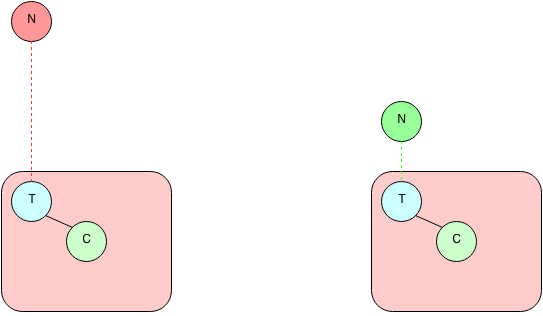
\includegraphics[width=0.65\textwidth]{img/algdesing/recombinationposib.png}
\caption{The possibilities for N to be moved. The right image is the better solution.} \end{figure}

To easily keep track of which rules a node is currently violating as well as facilitate the computation of fitness, each node keeps track of a byte field. 
The field acts as a register, each bit representing a certain rule. When the node violates a rule, the corresping is set to one. The usage of this register
structure relies on the fact that the number of rules is limited.

The last step is the edge routing. The method used is orthogonal edge routing. However, the process starts as a shortest path routing. The initial paths 
are direct lines between two nodes. Then, the paths are checked to see if they do not cross any obstacles. Should it cross another node, the path is split 
into orthogonal segments which go around the obstacle. This step is repeated until the path is clear of all obstacles and is incidental only to the source and 
destination. Lastly, should the drawn graph be planar, the drawing is checked for edge intersection. Paths which do not respect the planarity property 
are recomputed.
